
\section{Linear NN experiments}
Our main goal of this experiment is to test if deeper linear neural network can converge faster. we use linear MNIST with totally 60000 data points as our dataset. The first experiment randomly split this dataset into training set with 48000 training data points and 12000 test data points. The second experiment we use the full data as our training set.\\
Generally, we use a linear neural network model.  A linear NN with $H$ hidden layers can be modeled as
\begin{equation}
	\bm f(x,\bm\theta) = W_{H+1}(W_H(\cdots(W_1 x + b_1)\cdots)+b_H)+b_{H+1}
\end{equation}
where $W_1\in \mathbb{R}^{d_1\times d_x}$, $b_1 \in \mathbb{R}^{d_1}$, $W_i\in \mathbb{R}^{d_{i}\times d_{i-1}}$, $b_i \in \mathbb{R}^{d_i}$, $i = 2,\cdots,H$, $W_{H+1}\in \mathbb{R}^{d_y\times d_{H+1}}$, $b_{H+1} \in \mathbb{R}^{d_y}$. Notice that $d_x$ represents the input size which is 500 in this experiment, while $d_y$ represents the output size , namely, the number of classes, which is 10 in this experiment. So from now on, we may only  use an array $(d_x,d_1,\cdots,d_H,d_y)$ to represent our model.\\
We use cross-entropy with $L_2$ regularization as our loss function.
\begin{equation}
	L(\bm\theta,D) = \frac{1}{|D|} \sum_{i = 1}^k \sum_{x\in D_i} (\log ({\bm 1}^T e^{\bm f(x,\bm\theta)}) - f_i(x,\bm\theta)) + \lambda \sum_{j = 0}^{p+1} (\|W_j\|_F^2 + \|b_j\|_2^2)
\end{equation}

\begin{itemize}
	\item Model.\\
    \begin{itemize}
    	\item Net0 (500,10).
    	\item Net1 (500,100,10)
    	\item Net2 (500,200,100,10)
    	\item Net3 (500,400,200,100,10)
    	\item Net4 (500,800,200,100,10)
    \end{itemize}
    \item Training algorithm.
    \begin{itemize}
    	\item Full gradient descent(GD).
    	    \begin{equation}
    	    	\bm\theta = \bm\theta - lr \frac{\partial L}{\partial \bm\theta}
    	    \end{equation} 
    	\item Coordinate descent(CD).
    	\begin{align}
    		&\bm\theta_1^+ = \bm\theta_1 - lr \frac{\partial L}{\partial \bm\theta_1}(\bm\theta_1,\bm\theta_2,\cdots,\bm,\bm\theta_p,\theta_{p+1}),\\
    		&\bm\theta_2^+ = \bm\theta_2 - lr \frac{\partial L}{\partial \bm\theta_2}(\bm\theta_1^+,\bm\theta_2,\cdots,\bm\theta_p,\bm\theta_{p+1}),\\
    		&\bm\theta_3^+ = \bm\theta_3 - lr \frac{\partial L}{\partial \bm\theta_3}(\bm\theta_1^+, \bm\theta_2^+,\cdots,\bm\theta_p,\bm\theta_{p+1}),\\
    		&\cdots,\\
    		&\bm\theta_{p+1}^+ = \bm\theta_{p+1} - lr \frac{\partial L}{\partial \bm\theta_{p+1}}(\bm\theta_1^+, \bm\theta_2^+,\cdots,\bm\theta_p^+,\bm\theta_{p+1})
    	\end{align}
    	where $\bm\theta_j = (W_j,b_j), j = 1,2,\cdots,p+1$.
    \end{itemize}
    \item Stopping criterion.\\
    We stop iteration when training accuracy first obtain 100\%.
\end{itemize}


\newpage
\begin{enumerate}
	\item Training Net0-4 using gradient descent.\\
	We set $\lambda = 10^{-5}$, learning rate $= 0.1$.
	\begin{itemize}
		\item Experiment 1: Using ranomly chosen 48000 data points from linear MNIST as training set.\\
		\begin{table}[H]
			\centering
			\caption{Randomly chosen 80\% full dataset as training set}
			\label{tab:1}      
			\begin{tabular}{lllllll}
				\hline\noalign{\smallskip}
				Model &  Optim & Iterations & Time  & TrainL  & TestL & TestA \\
				\noalign{\smallskip}\hline\noalign{\smallskip}
				
				Net0 & GD & 3190 & 3743 & 0.0062 & 0.0077 & 99.94   \\
				
				Net1 & GD & 2009 & 2475 & 0.0046 & 0.0063 & 99.95 \\
				
				Net2 & GD & 2322 & 3245 & 0.0034 & 0.0049 & 99.94 \\
				
				Net3 & GD & 1767 & 2705 & 0.0048 & 0.0066 & 99.93 \\
				
				Net4 & GD & 1805 & 3346 &0.0059 & 0.0075 & 99.93 \\
				
				\noalign{\smallskip}\hline
				
			\end{tabular}
		\end{table}
		
		\begin{figure}[H]
			\centering
			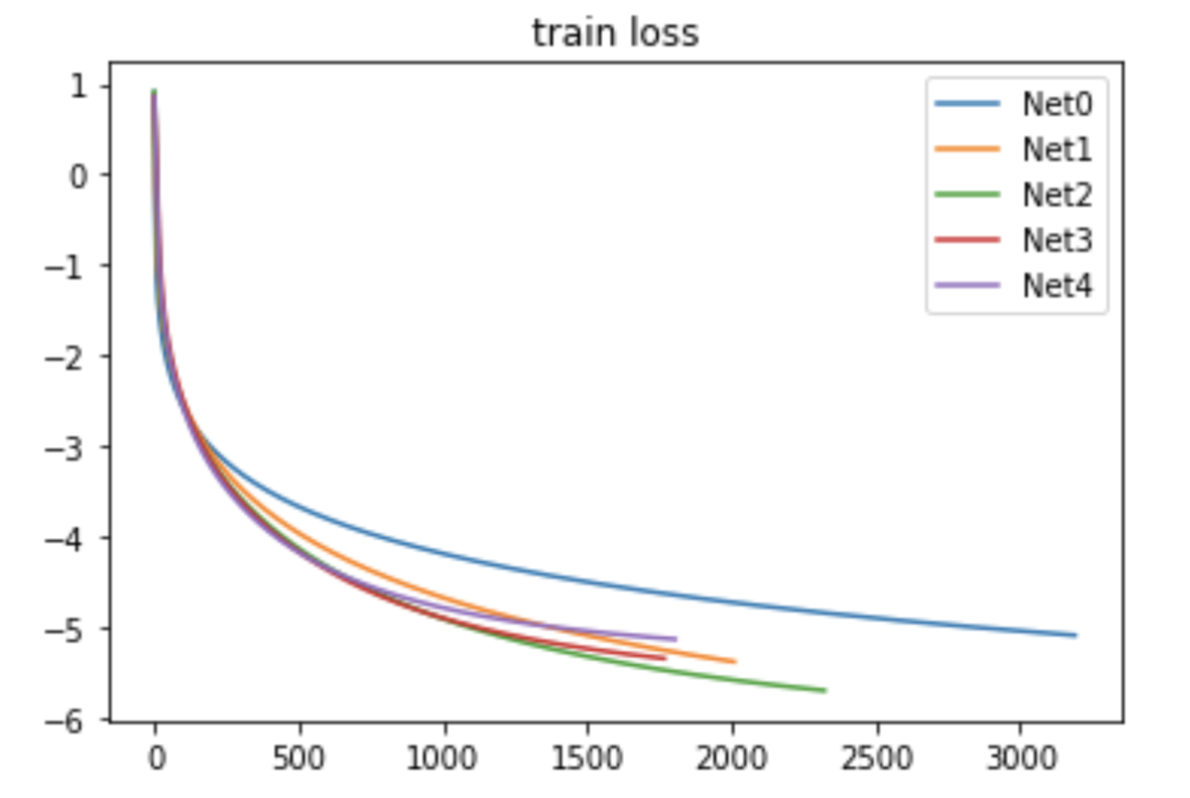
\includegraphics[width=3in]{figure/logGDtrainL.png}   
			\caption{log(Train Loss)}
		\end{figure}

	
	
	
		\item Experiment 2: Using whole linear MNIST dataset as training set.
		\begin{table}[H]
			\centering
			\caption{Full dataset}
			\label{tab:2}      
			\begin{tabular}{lllll}
				\hline\noalign{\smallskip}
				Model &  Optim & Iterations & Time  & TrainL \\
				\noalign{\smallskip}\hline\noalign{\smallskip}
				
				Net0 & GD & 4218 & 6168 & 0.0051  \\
				
				Net1 & GD & 2546 & 3937 & 0.0038  \\
				
				Net2 & GD & 2269 & 4010 & 0.0035  \\
				
				Net3 & GD & 2099 & 4046 & 0.0044  \\
				
				Net4 & GD & 1578 & 3815 &0.0065  \\
				
				\noalign{\smallskip}\hline
				
			\end{tabular}
		\end{table}
		
		
		\begin{figure}[H]
			\centering
			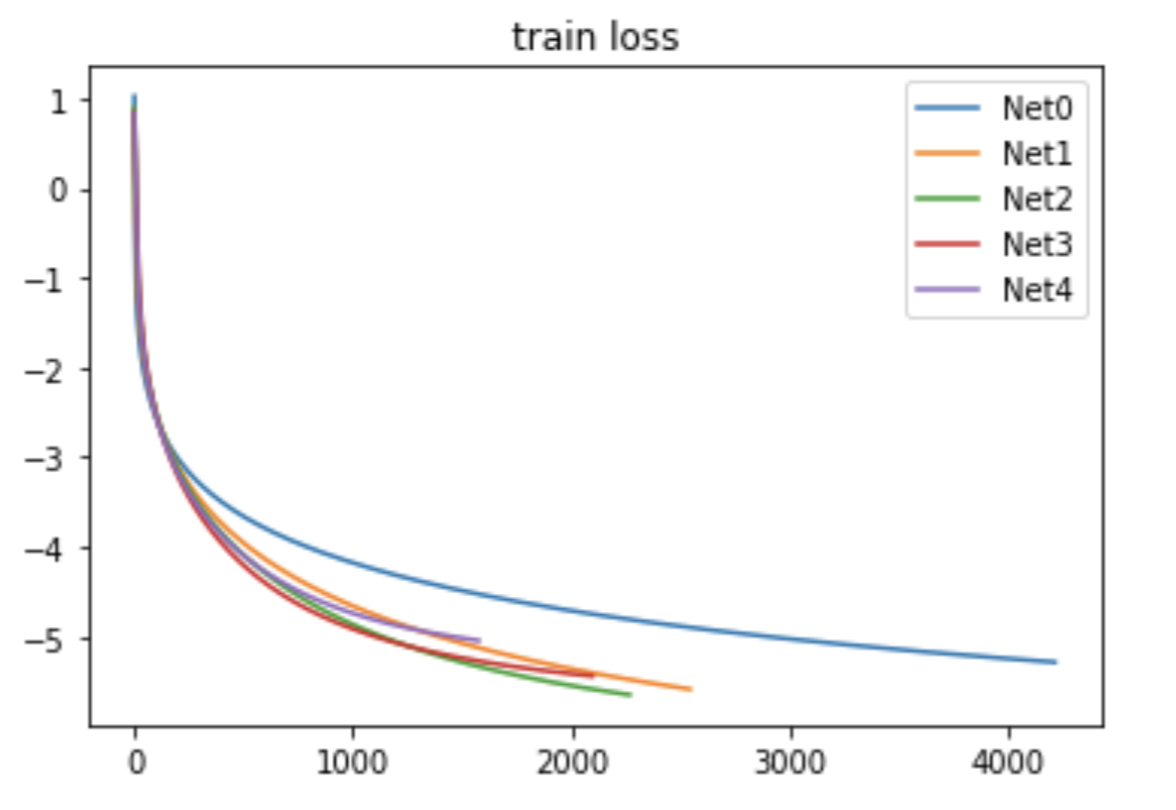
\includegraphics[width=3in]{figure/logGDfullL.png}   
			\caption{log(Train Loss) for full dataset}
		\end{figure}
		We can see very clearly in the two figures that the loss of Net0 always decrease slower than other deeper linear NN. Or we can see in the table that Net0 use most iterations to reach 100\% training accuracy. 
	
	    \item Experiment 3: Training '0' and '1' data in MNIST.\\
	     First I use Adam algorithm to verify that '0' and '1' are linearly separable in the training set of MNIST. Then I use full GD to iterate 50 epoches for each model and record their loss history. 
	    \begin{figure}[H]
		  \centering
		  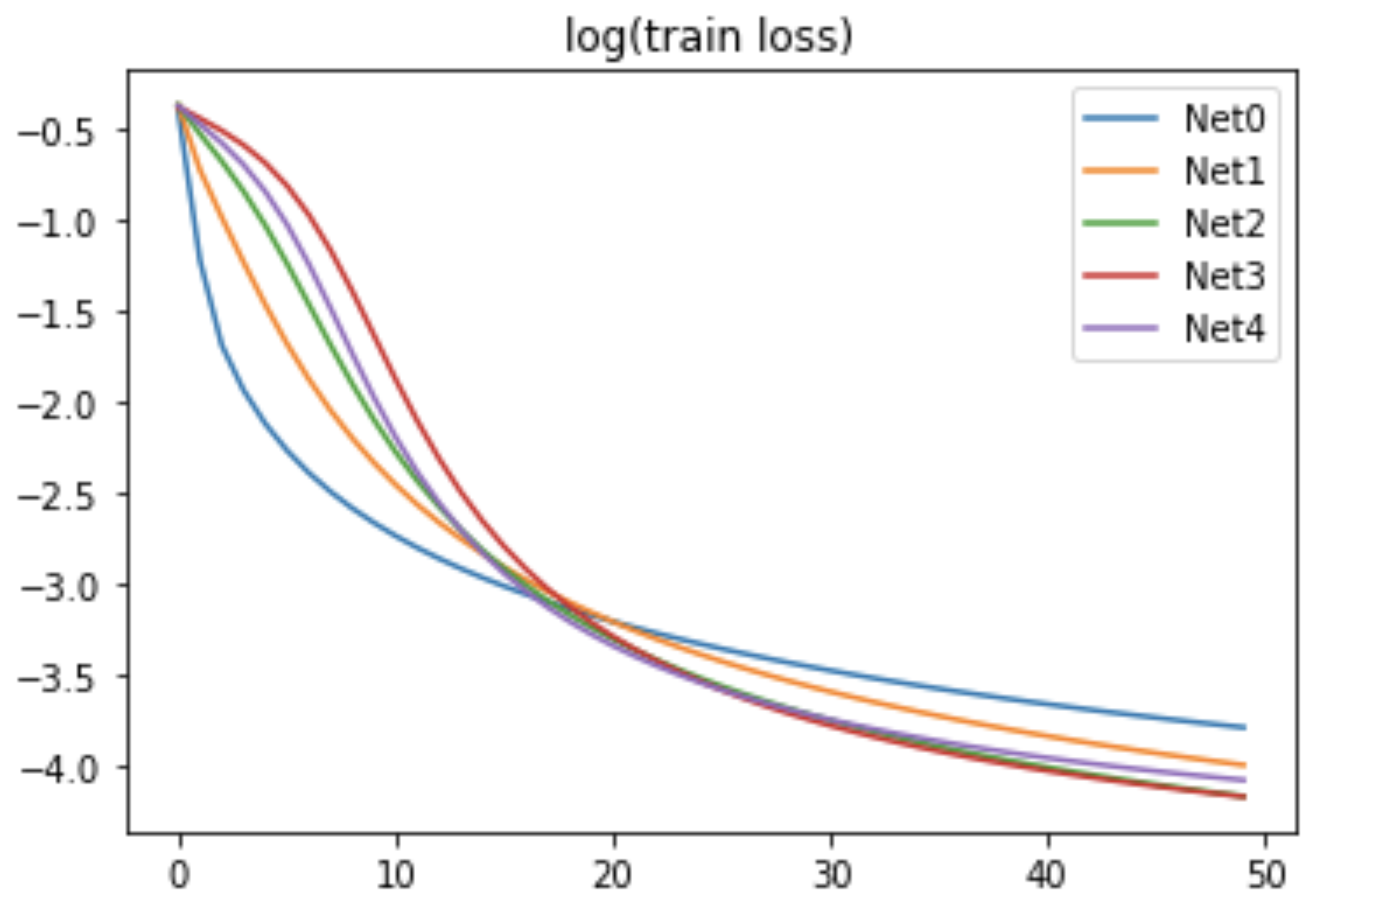
\includegraphics[width=3in]{figure/log_MNIST_50.png}   
		  \caption{log(Train Loss) for MNIST dataset}
	      \end{figure}
		\end{itemize}
	\end{enumerate}

		
     
	
	





\newpage
\section{A new training algorithm}
\begin{figure}[H]
	\centering
	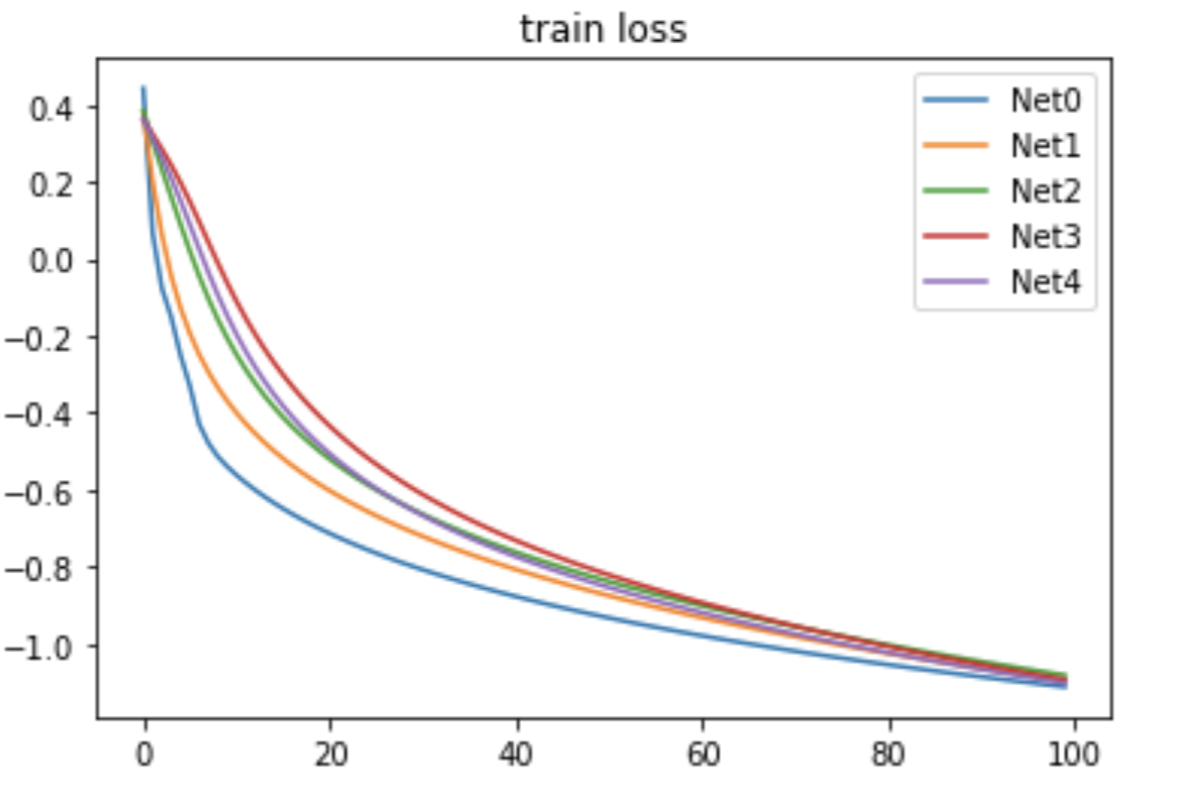
\includegraphics[width=3in]{figure/part_logGDfullL.png}   
	\caption{part of log(Train Loss) for full dataset}
\end{figure}

If we print the first several steps, we will notice that the loss of Net0 descends the fastest among those networks. After 5-10 steps, it suddenly become the slowest. If at this point we can switch to another curve, then the training process might speed up.\\

\subsection{Regression training}
Actually, there is two ways to achieve this. We may use a very simple regression example to discribe those two methods. We denote our training data as $X\in \mathbb{R}^{d_x\times N}$, the label is $Y\in \mathbb{R}^{d_y\times N}$. Basically, our model is the simplest linear model
\begin{equation}
	f(x) = Wx,
\end{equation}
and our loss function is 
\begin{equation}
	L(W, D) = \|WX - Y\|_F^2.
\end{equation}
First, we use 
\begin{equation}
	W = W - lr \frac{\partial L}{\partial W}
\end{equation}
to do several iterations to obtain $\overline{W}$. Then we have three ways to continue.\\
\begin{itemize}
	\item Reformulate the problem as 
	\begin{equation}
	\min_{U,V} \|(\overline{W}+ UV)X - Y\|_F^2
	\end{equation}
	where $U\in \mathbb{R}^{d_y\times d_1}$, $V\in\times \mathbb{R}^{d_1\times d_x}$. If the solution of above problem is $\overline{U}, \overline{V}$, then our final solution is $W = \overline{W}+\overline{U}\overline{V}$. Notice that if we use a zero initialization in the above problem, the begining loss is $\|\overline{W} X - Y\|_F^2$.\\
	\item Factorize $\overline{W} = U_0 V_0$, where $\overline{U}_0\in \mathbb{R}^{d_y\times d_1}$, $\overline{V}_0\in\times \mathbb{R}^{d_1\times d_x}$. And we use $(U_0,V_0)$ as the initial value for the following problem:
	\begin{equation}
	\min_{U,V} \|UVX - Y\|_F^2.
	\end{equation}
	If the solution of above problem is $\overline{U}, \overline{V}$, then our final solution is $W = {\overline{U}}{\overline{V}}$.
\end{itemize}

\subsection{Classification Training}
For classification problem, we have three possible ways to speed up the training algorithms. Define function $l: \mathbb{R}^{d_x}\times \{1,2,\cdots,d_y\} \rightarrow \mathbb{R}$ as
\begin{equation}
	l(\bm s, i) = \log ({\bm 1}^T e^{\bm s}) - s_i,
\end{equation}
where $\bm s = (s_1,s_2,\cdots,s_{d_y})$. So our final cross-entropy loss can be written as
\begin{equation}
	L(\bm\theta,D) = \sum_{i = 1}^{d_y} \sum_{x\in D_i} l(f(x), i) 
\end{equation}
where $f$ is the mapping of our model.  
We use single-layer and 2-layer linear NN as our examples to state our possible ways to speed up training. For single-layer linear NN we use $W,b$ to represents the weight matrix and bias vector, so $f(x) = Wx + b$. For 2-layer linear NN we use $W_1,W_2,b$ to represents the 2 weight matrices and the bias vector , and $f(x) = W_2 W_1 x + b$ (which implies the first layer is without bias).\\

There are 3 main ideas of speed-up training algorithms.
\begin{itemize}
	\item  Use single-layer linear NN and cross-entropy loss to do several iterations to get parameter $\overline{W}, \overline{b}$. Then we modify the optimization problem as
	\begin{equation}
		\min_{W_1,W_2,b}\sum_{i = 1}^{d_y} \sum_{x\in D_i} l((\overline{W}+W_2 W_1)x + (\overline{b}+b), i) 
	\end{equation}
	If $\tilde{W}_1,\tilde{W}_2,\tilde{b}$ is one of the solution of the above problem, then our final solution is $W^* = \overline{W} + \tilde{W}_2\tilde{W}_1, b^* = \overline{b} + \tilde{b}$.\\
	
	\item In the second training algorithm, we use a 2-layer linear NN all the time. The loss is 
	\begin{equation}
	\sum_{i = 1}^{d_y} \sum_{x\in D_i} l(W_2 W_1x + b, i) 
	\end{equation}
	 But in first several steps, we fix the initial $W_1$, only update $W_2$ and $b$. If you regard $W_1 x$ as a whole, we can see we are actually training a single-layer linearNN at the begining. After several steps, we start to update $W_1,W_2,b$ together just as the regular GD.\\
	 
	 \item The third idea is, just like the first idea, we use single-layer linear NN and cross-entropy loss to do several iterations to get parameter $\overline{W}, \overline{b}$. But after that, we factorize $\overline{W} = U_0 V_0$, where $\overline{U}_0\in \mathbb{R}^{d_y\times d_1}$, $\overline{V}_0\in\times \mathbb{R}^{d_1\times d_x}$. And we use $W_2 = U_0, W_1 = V_0, b = \overline{b}$ as the initial value for the following problem:
	 \begin{equation}
	 \min_{W_1,W_2,b} \sum_{i = 1}^{d_y} \sum_{x\in D_i} l(W_2 W_1x + b, i) .
	 \end{equation}

	 
\end{itemize}

\subsubsection{Idea I}
\begin{figure}[H]
	\centering
	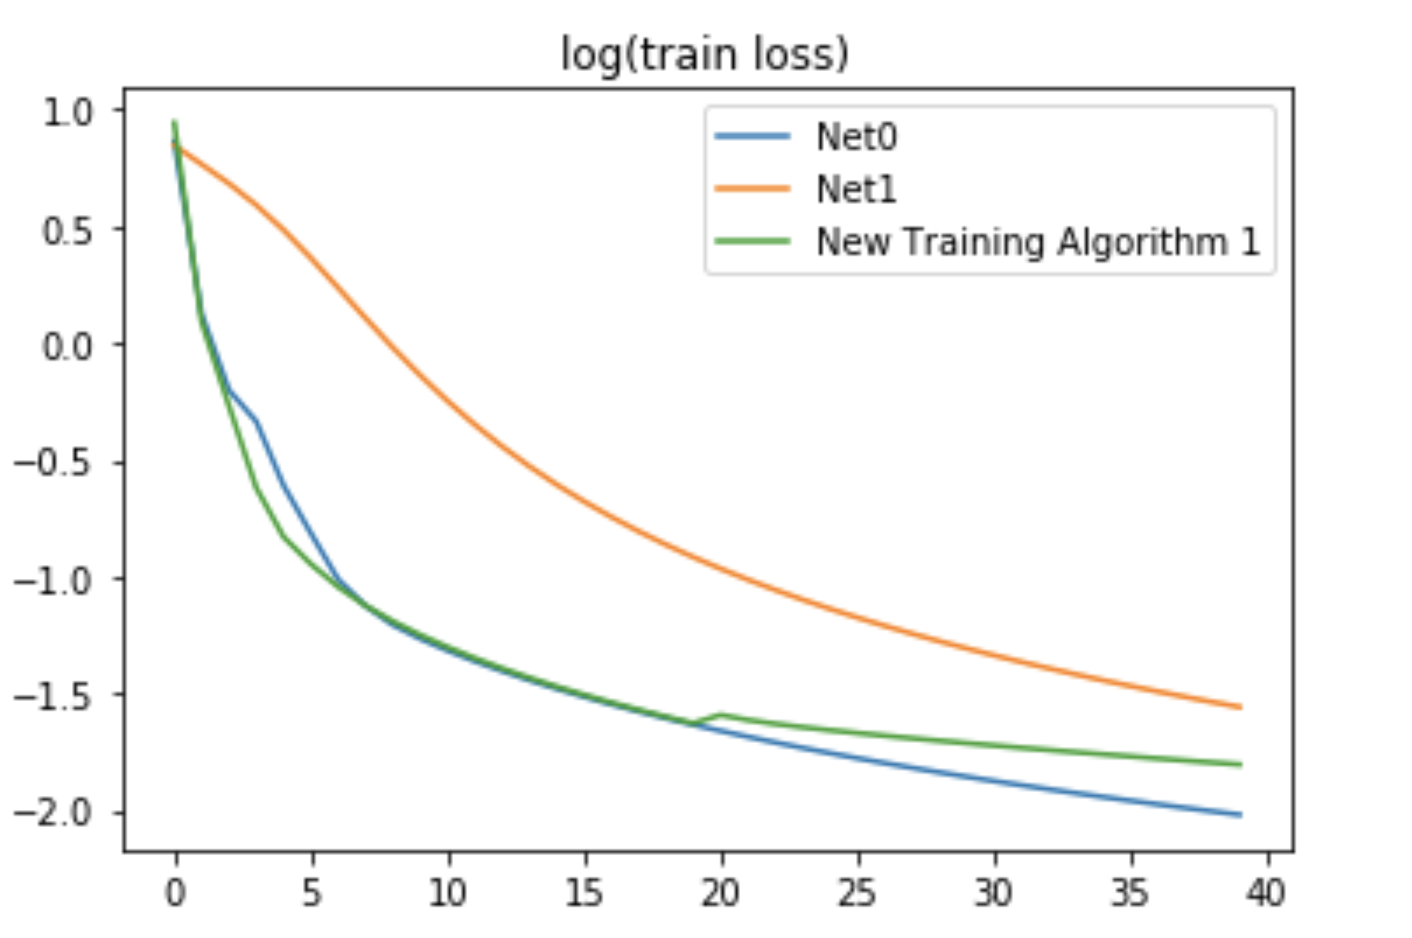
\includegraphics[width=2.5in]{figure/train1_hidden100.png}
	\caption{New training algorithm 1: $d_1 = 100, lr = 0.1$}
\end{figure}
\begin{figure}[H]
	\centering
	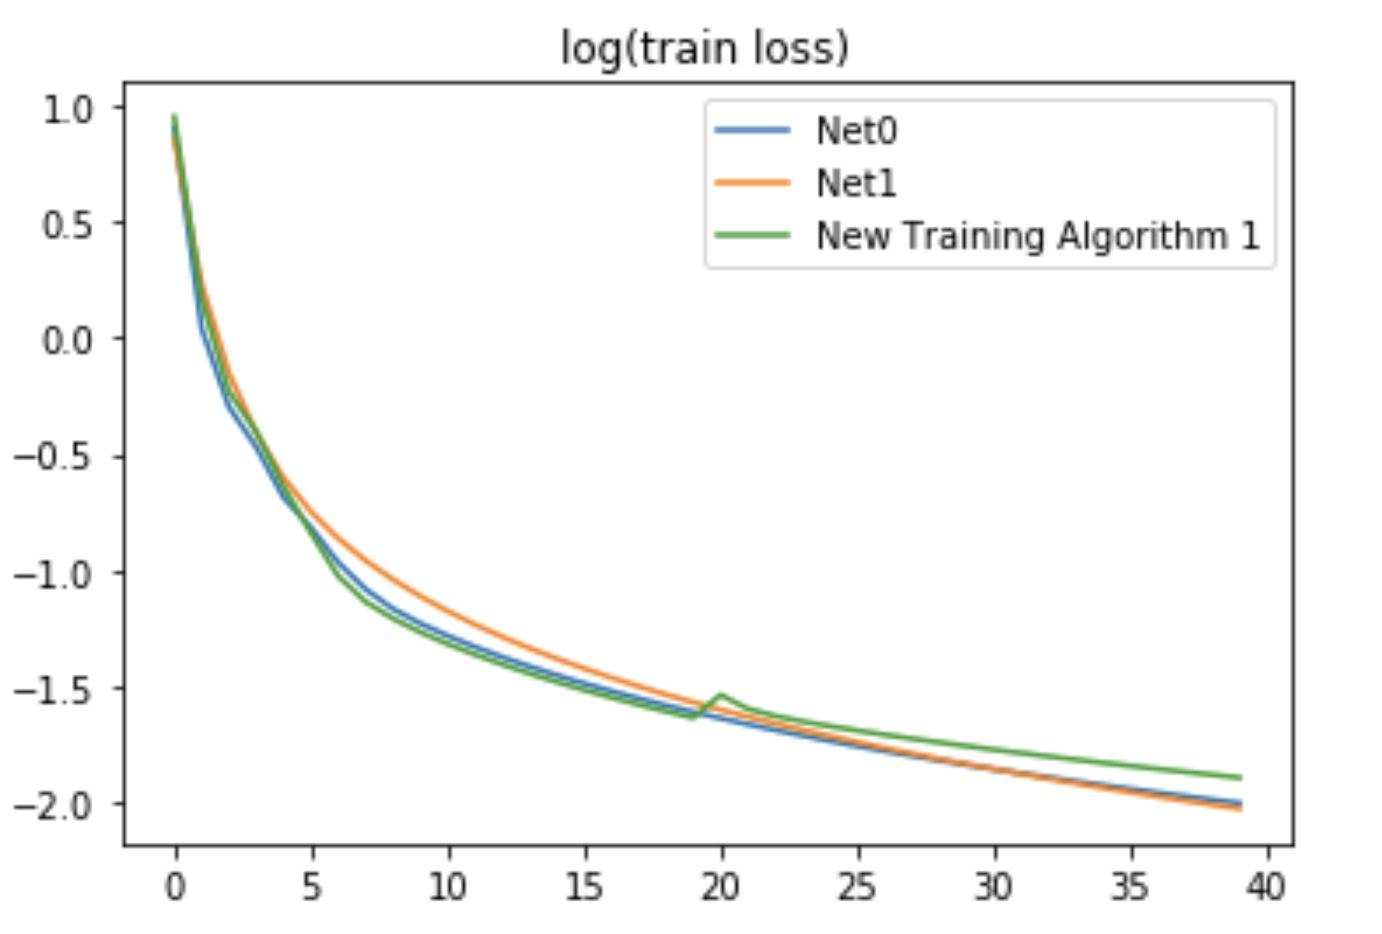
\includegraphics[width=2.5in]{figure/train1_hidden500.png}
	\caption{New training algorithm 1: $d_1 = 500, lr = 0.1$}
\end{figure}
Here we found that when we switch to the 2-layer model, the descent speed becomes slower.

\subsection{Idea II}
\begin{figure}[H]
	\centering
	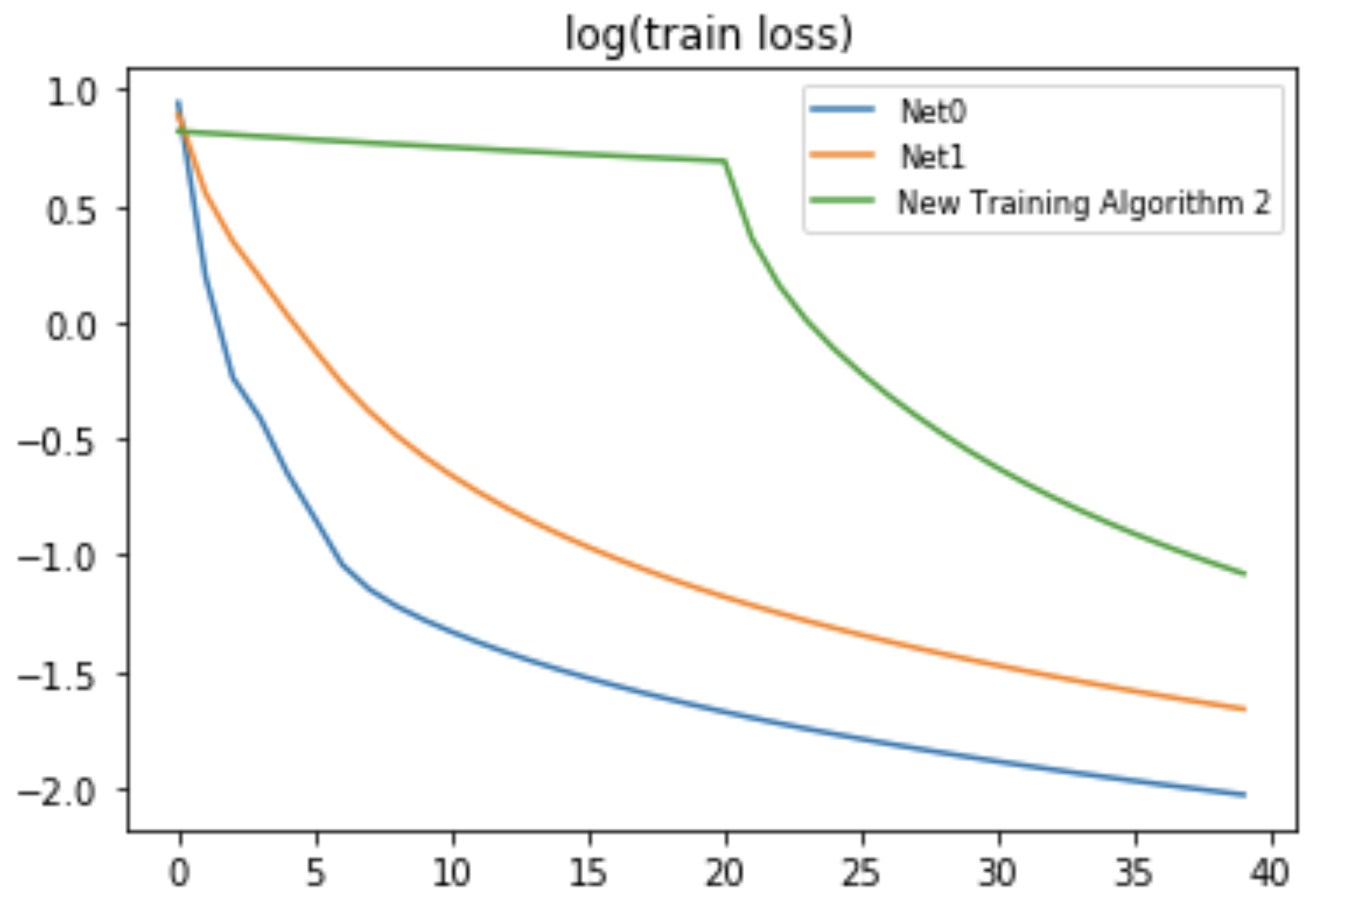
\includegraphics[width=2.5in]{figure/train2_hidden10.png}
	\caption{New training algorithm 2: $d_1 = 10, lr = 0.1$}
\end{figure}
\begin{figure}[H]
	\centering
	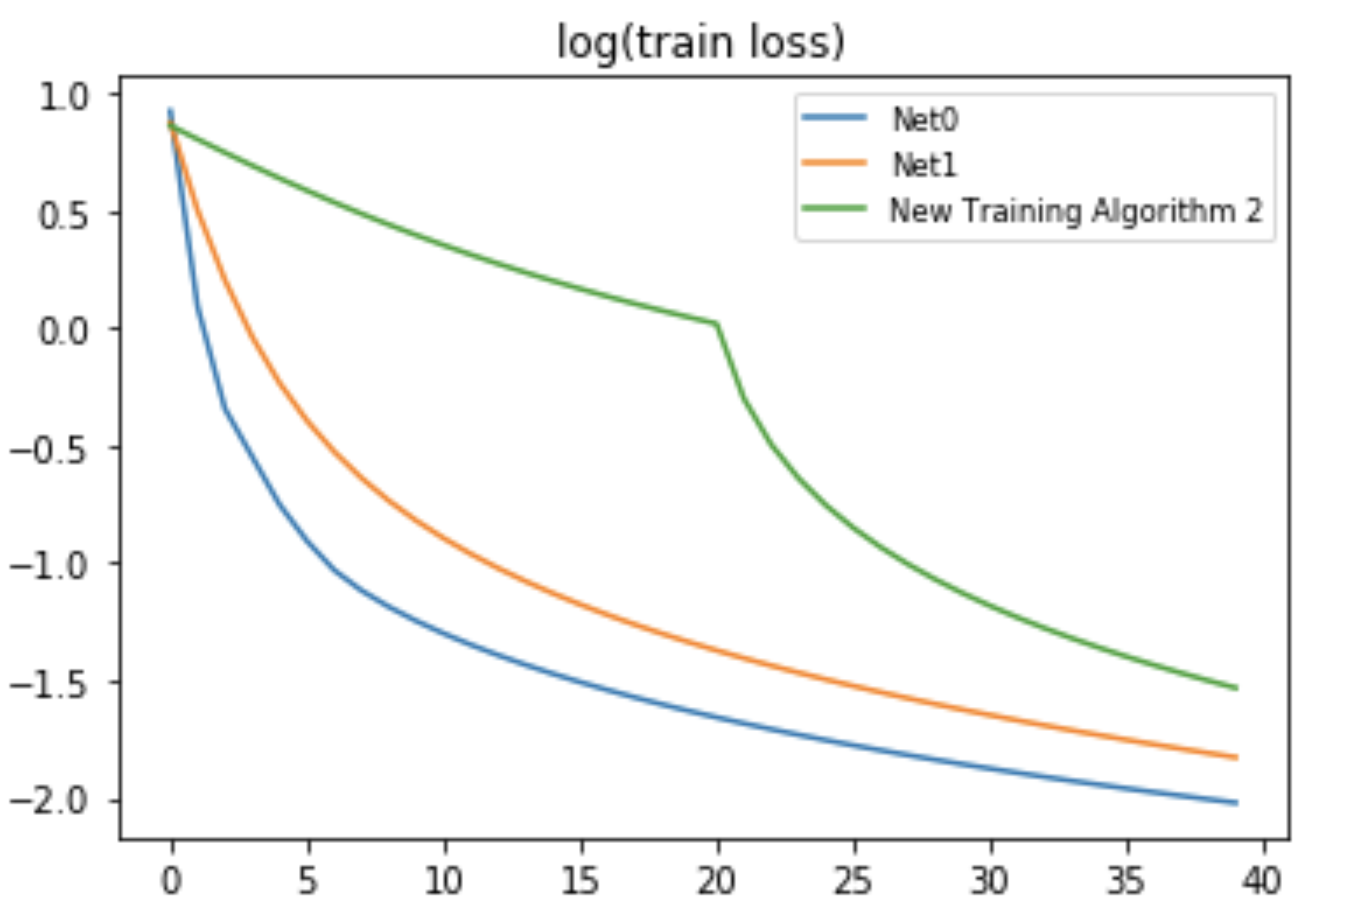
\includegraphics[width=2.5in]{figure/train2_hidden100.png}
	\caption{New training algorithm 2: $d_1 = 100, lr = 0.1$}
\end{figure}
\begin{figure}[H]
	\centering
	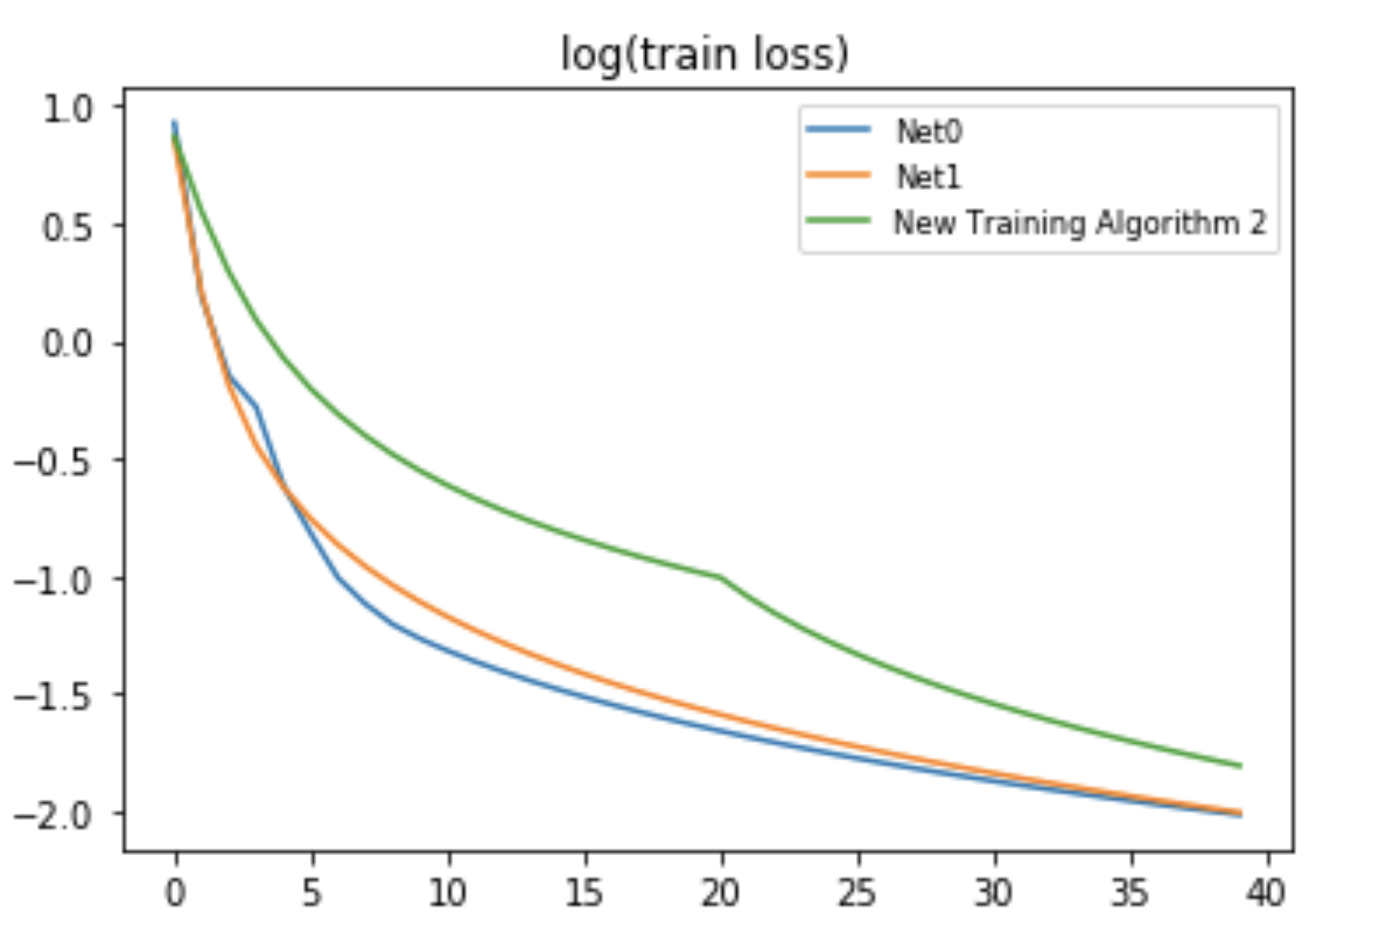
\includegraphics[width=2.5in]{figure/train2_hidden500.png}
	\caption{New training algorithm 2: $d_1 = 500, lr = 0.1$}
\end{figure}
\begin{figure}[H]
	\centering
	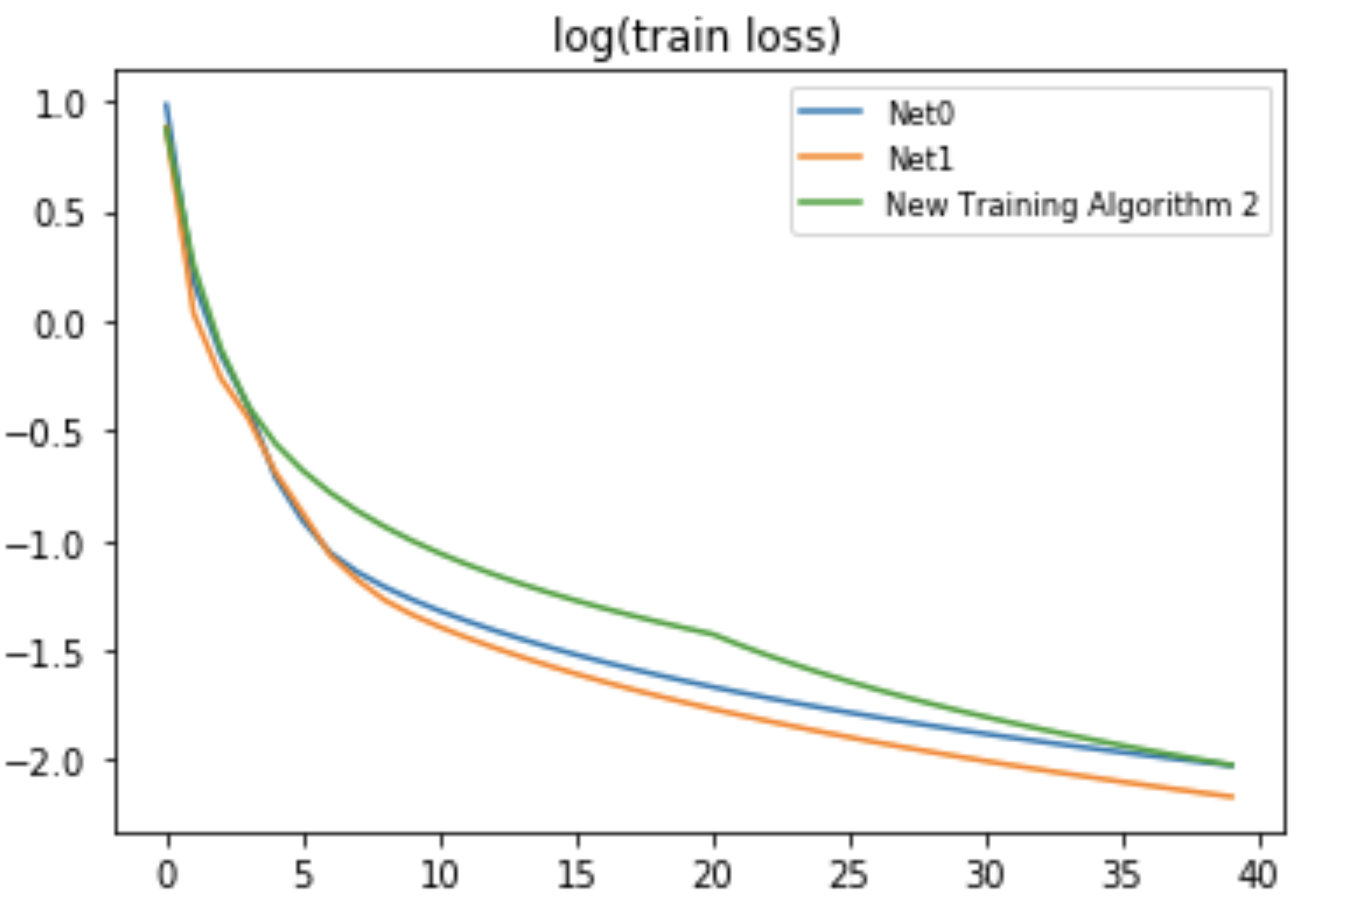
\includegraphics[width=2.5in]{figure/train2_hidden1000.png}
	\caption{New training algorithm 2: $d_1 = 1000, lr = 0.1$}
\end{figure}
\begin{figure}[H]
	\centering
	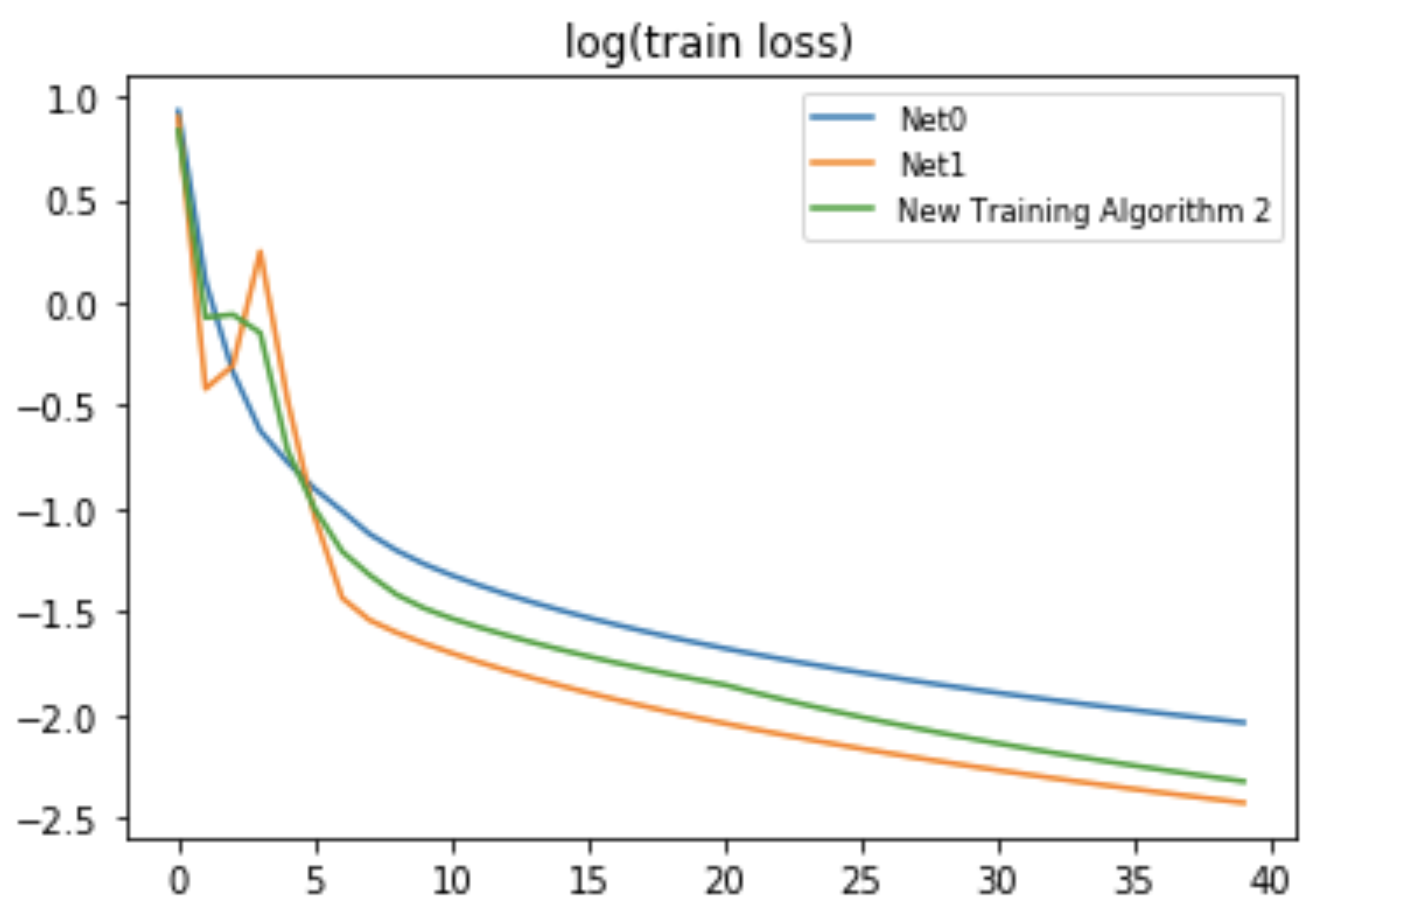
\includegraphics[width=2.5in]{figure/train2_hidden2000_lr1.png}
	\caption{New training algorithm 2: $d_1 = 2000, lr = 0.1$}
\end{figure}
\begin{figure}[H]
	\centering
	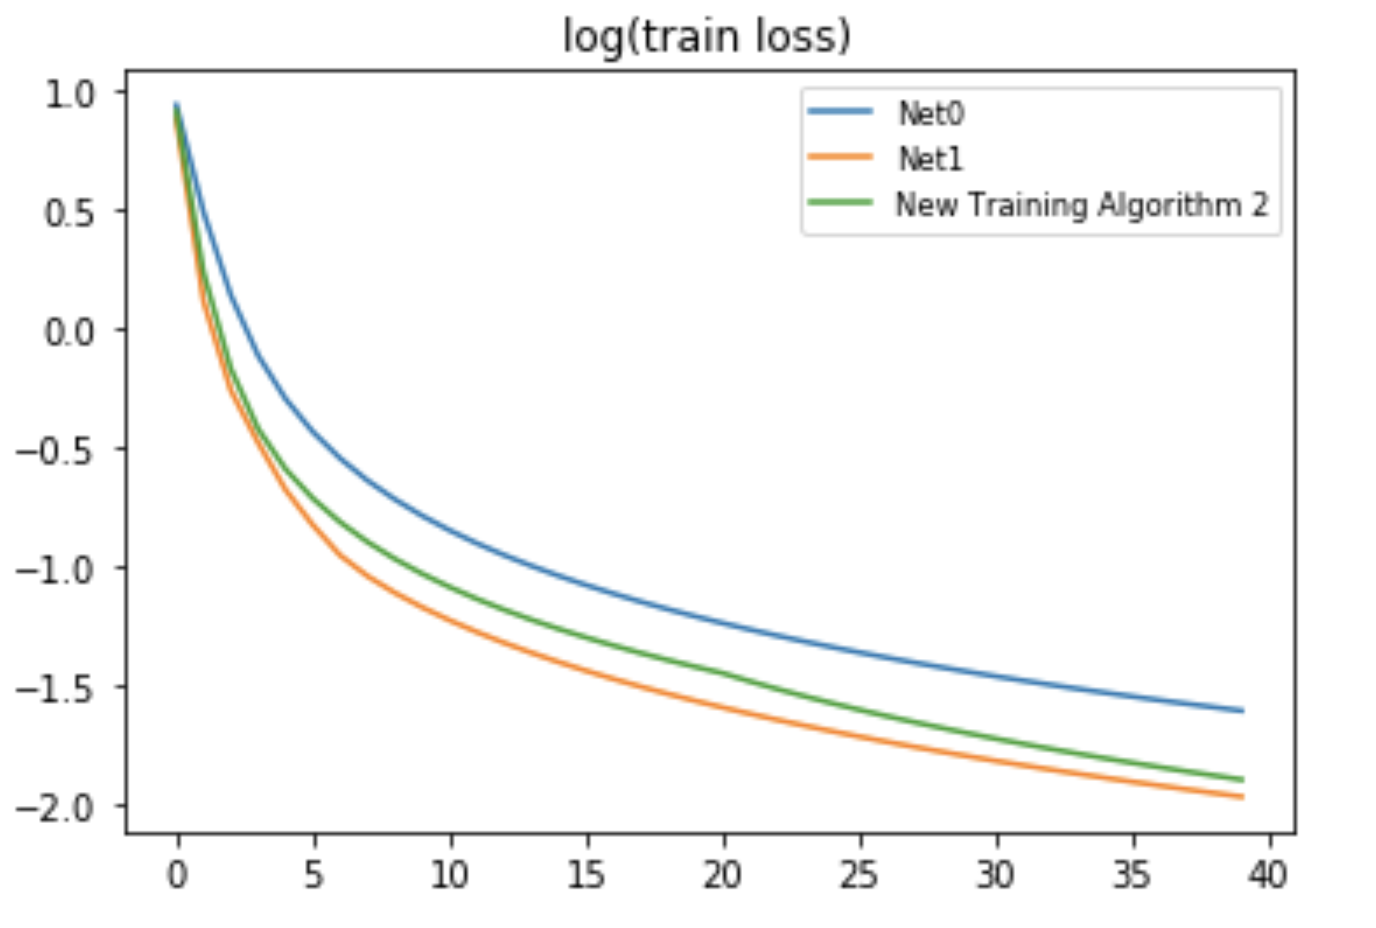
\includegraphics[width=2.5in]{figure/train2_hidden2000_lr05.png}
	\caption{New training algorithm 2: $d_1 = 2000, lr = 0.05$}
\end{figure}

Here are some interesting things we can observe:
\begin{itemize}
	\item It seems that idea II do have an acceleration at 20th iteration (bacause we start to update all parameters that step), but the descending speed is slower than Net0 in the first 20 steps when the hidden size is less than 500.
	\item When we increase the hidden size to 1000 or 2000, our idea do descend faster than Net0 at the beginning, but slower than Net1. So our idea II seems useless when size of hidden-layer is very large.

	
\end{itemize}

An interesting phenomenon is that if we increase the size of the hidden layer, the two-layer linear NN descend faster from the beginning than single-layer linear NN. We use 0 and 1 in MNIST dataset to observe if this phenomenon also occurs in MNIST dataset.

\begin{figure}[H]
	\centering
	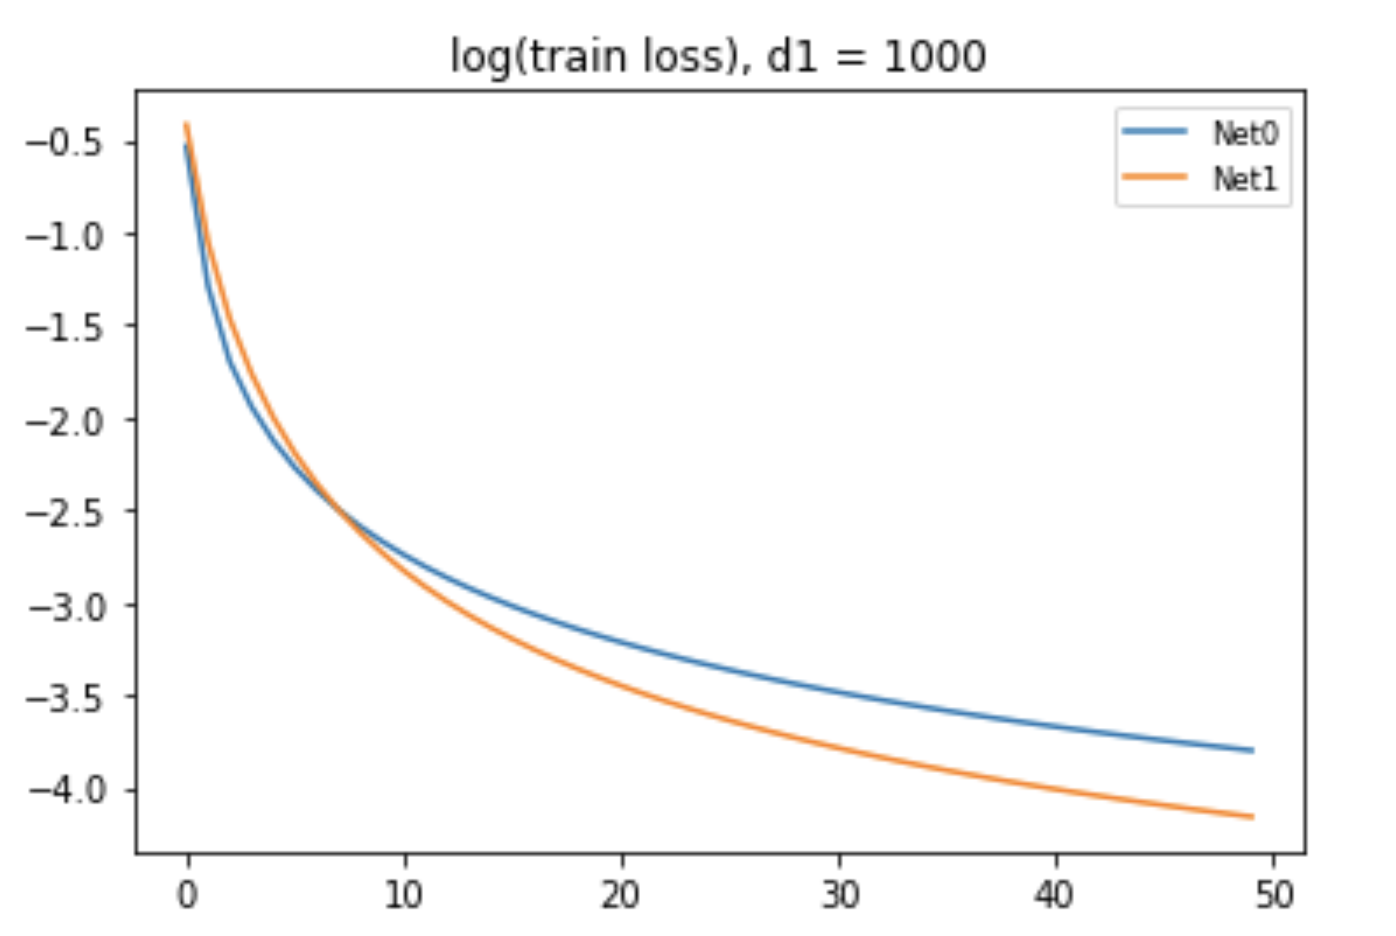
\includegraphics[width=2.5in]{figure/MNIST_hidden1000_step50.png}
	\caption{MNIST: $d_1 = 1000, lr = 0.1$}
\end{figure}


\begin{figure}[H]
	\centering
	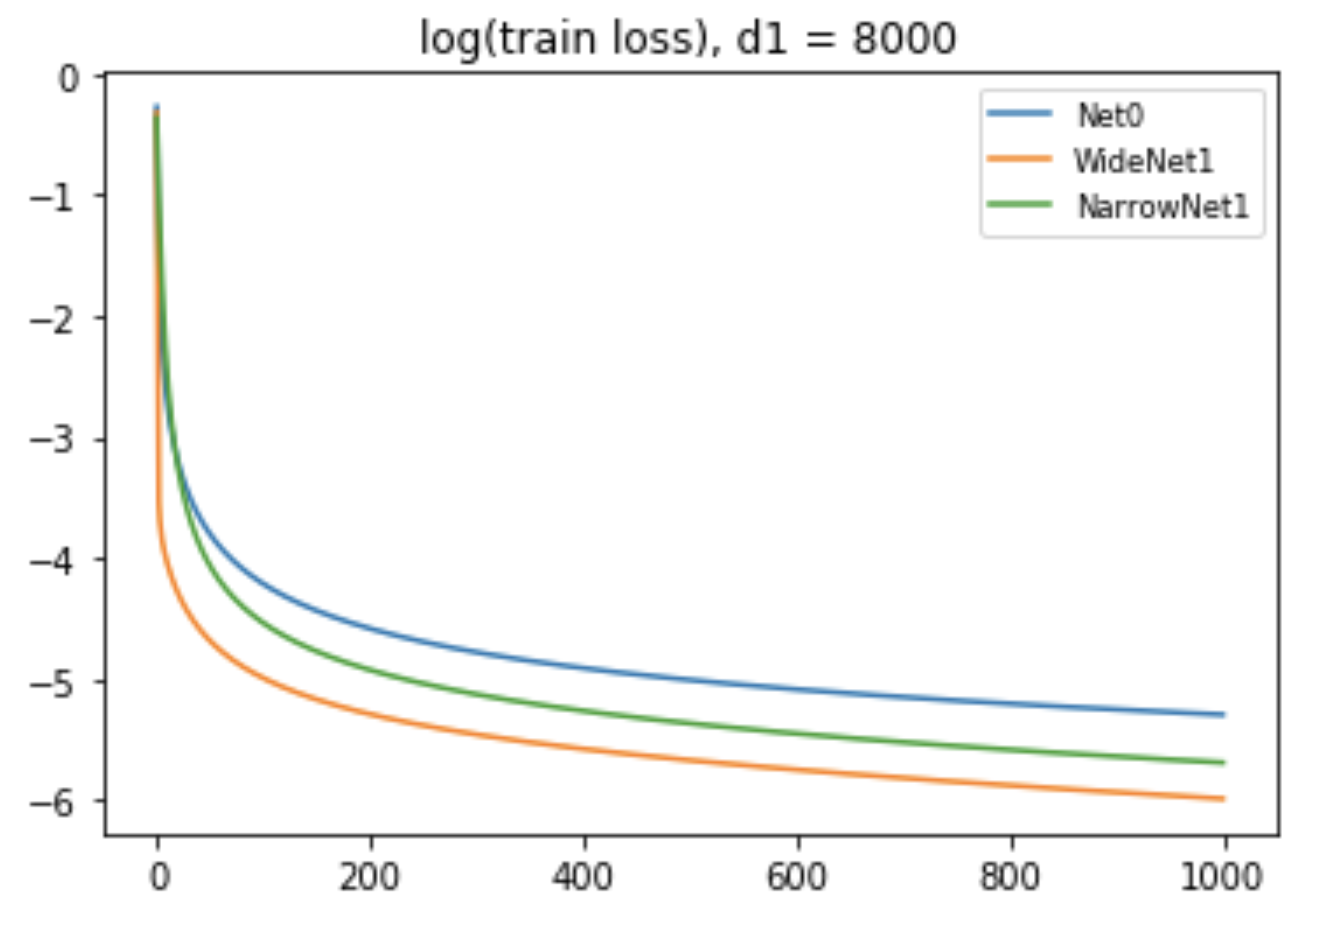
\includegraphics[width=2in]{figure/MNIST_hidden8000_step1000.png}
	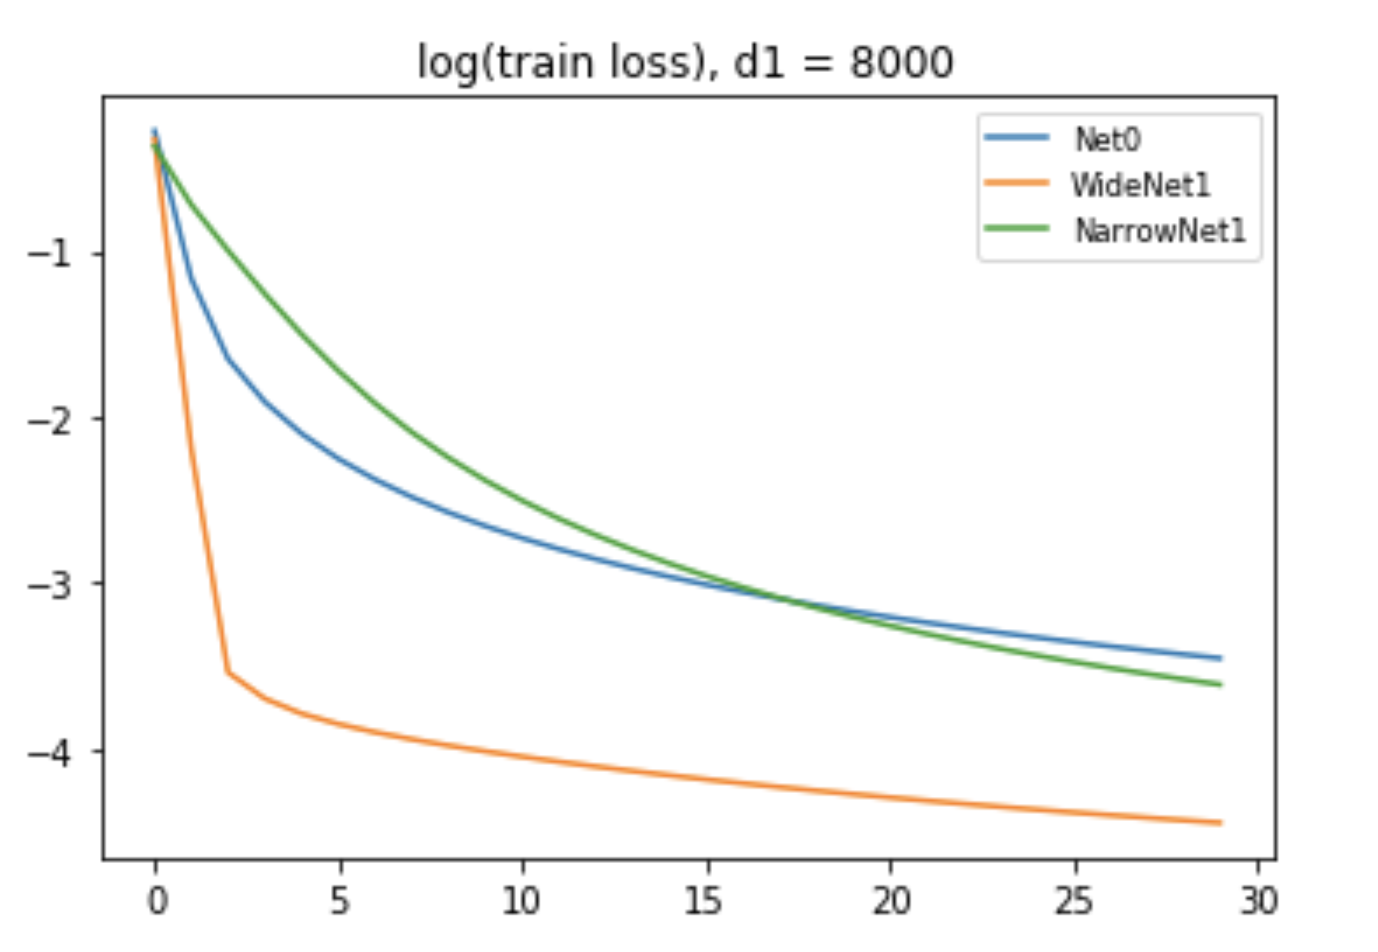
\includegraphics[width=2in]{figure/MNIST_hidden8000_step30.png}
	\caption{MNIST: WideNet($d_1 = 8000$) vs NarrowNet($d_1 = 100$)}
\end{figure}

\begin{figure}[H]
	\centering
	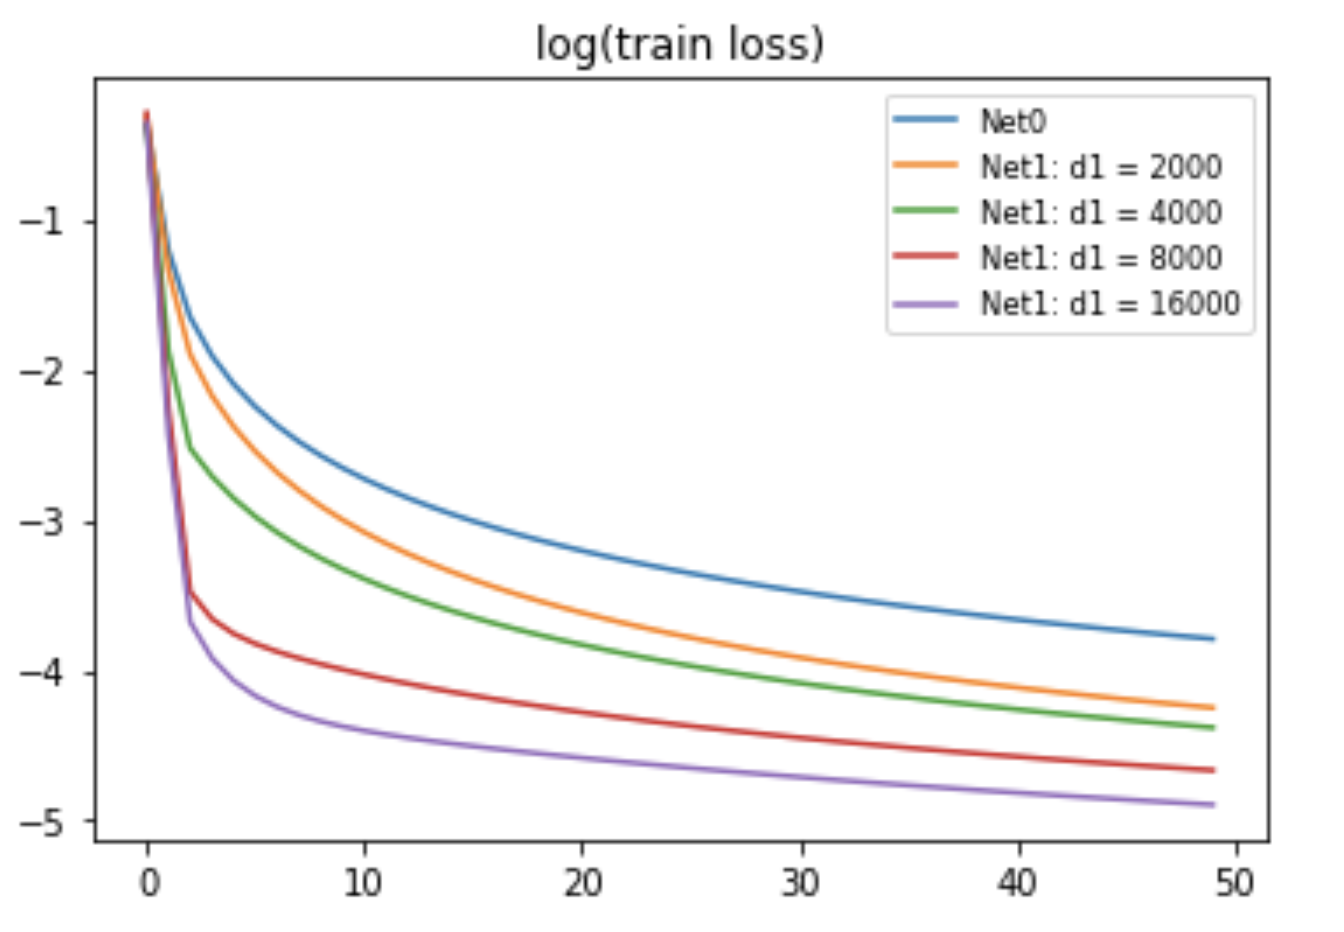
\includegraphics[width=2in]{figure/MNIST_hidden64000_1.png}
	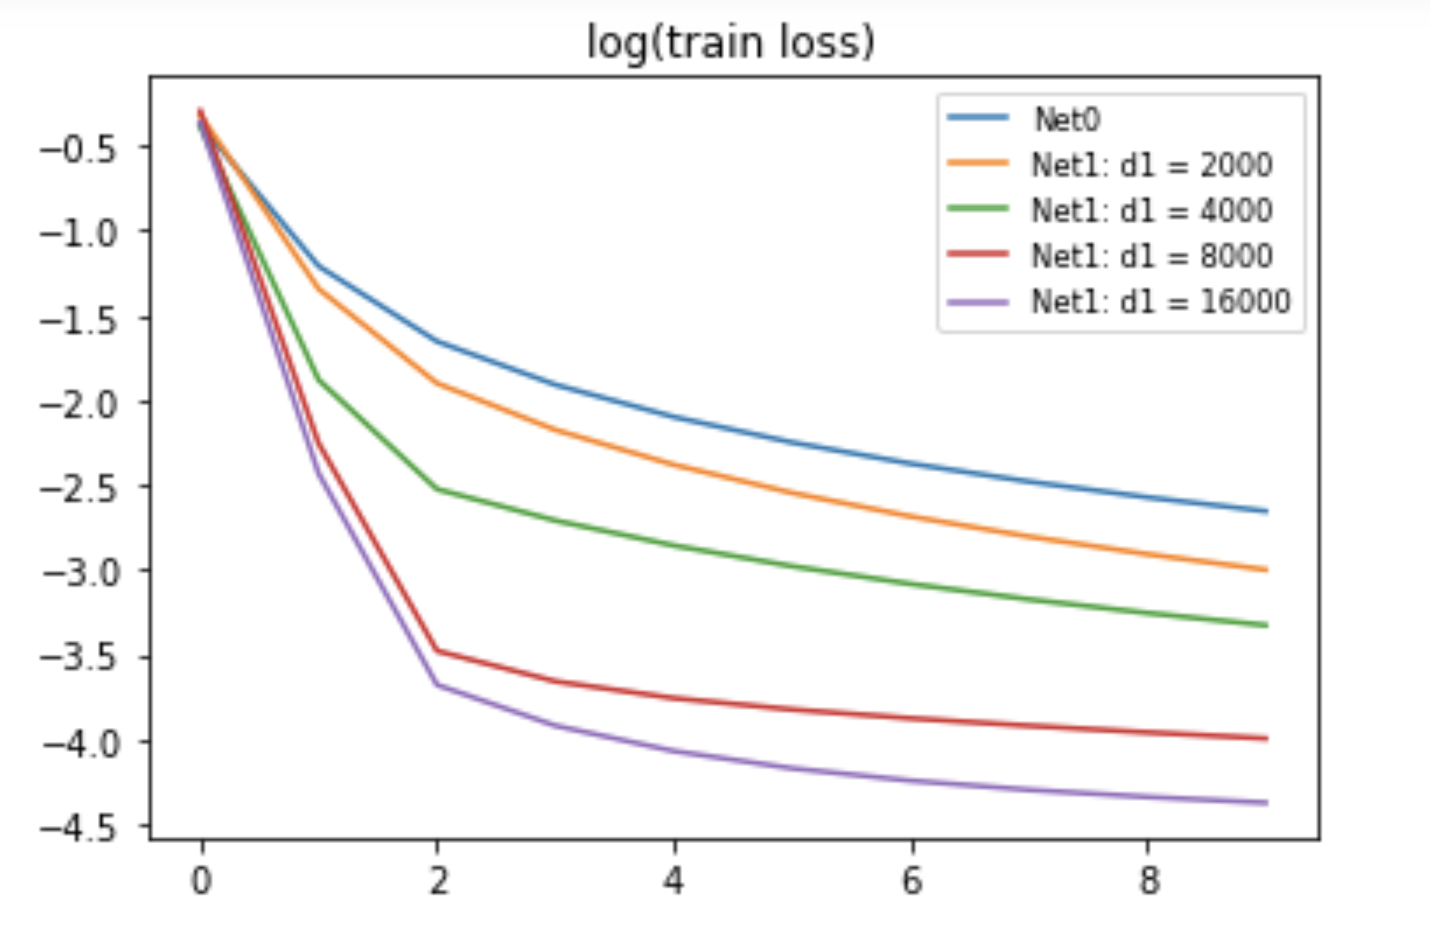
\includegraphics[width=2in]{figure/MNIST_hidden64000_2.png}
	\caption{MNIST: $d_1 = 2000,4000,8000,16000$}
\end{figure}

\begin{figure}[H]
	\centering
	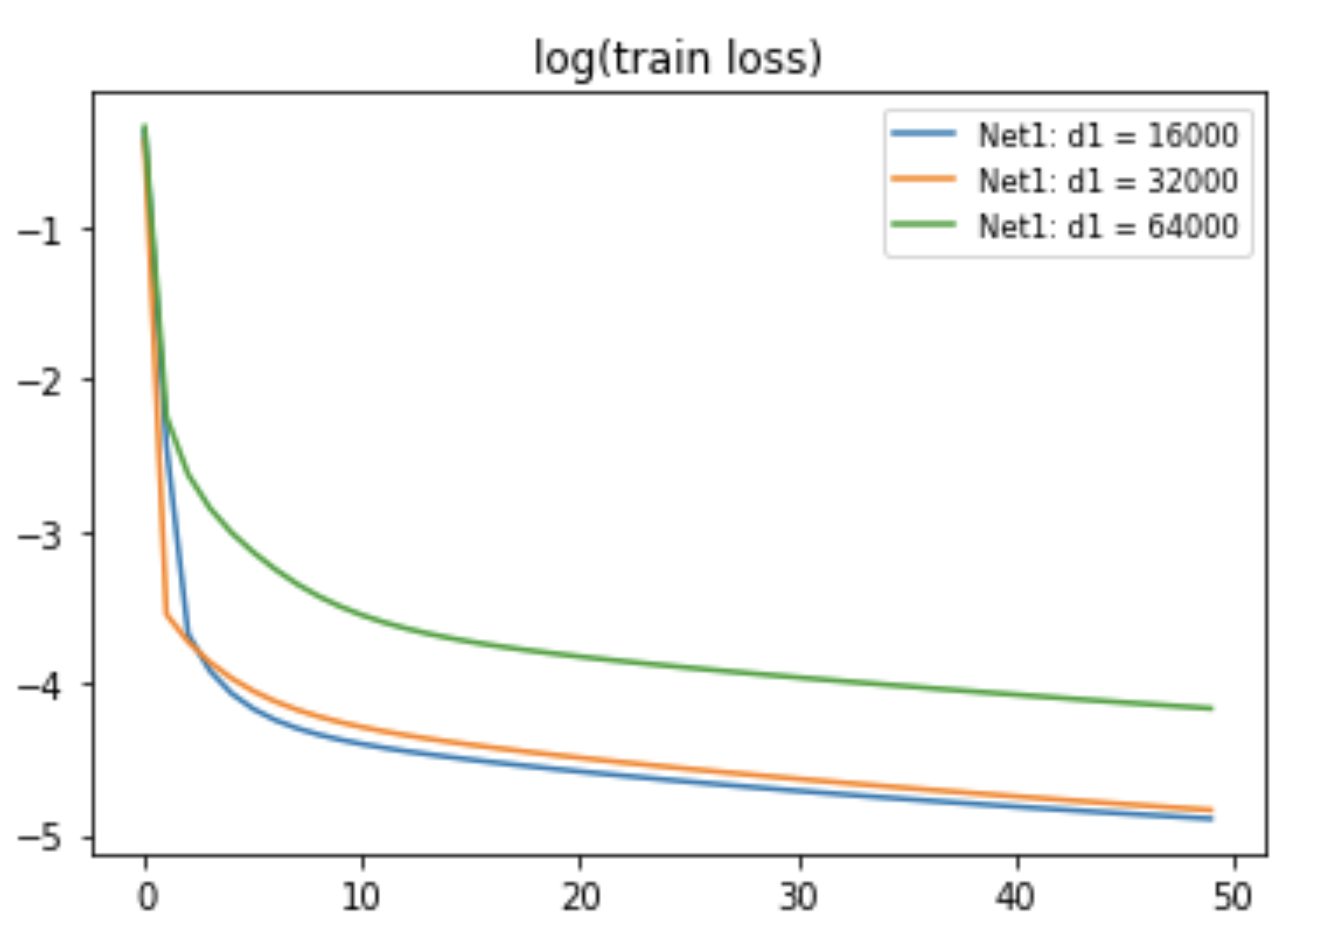
\includegraphics[width=2in]{figure/MNIST_hidden64000_3.png}
	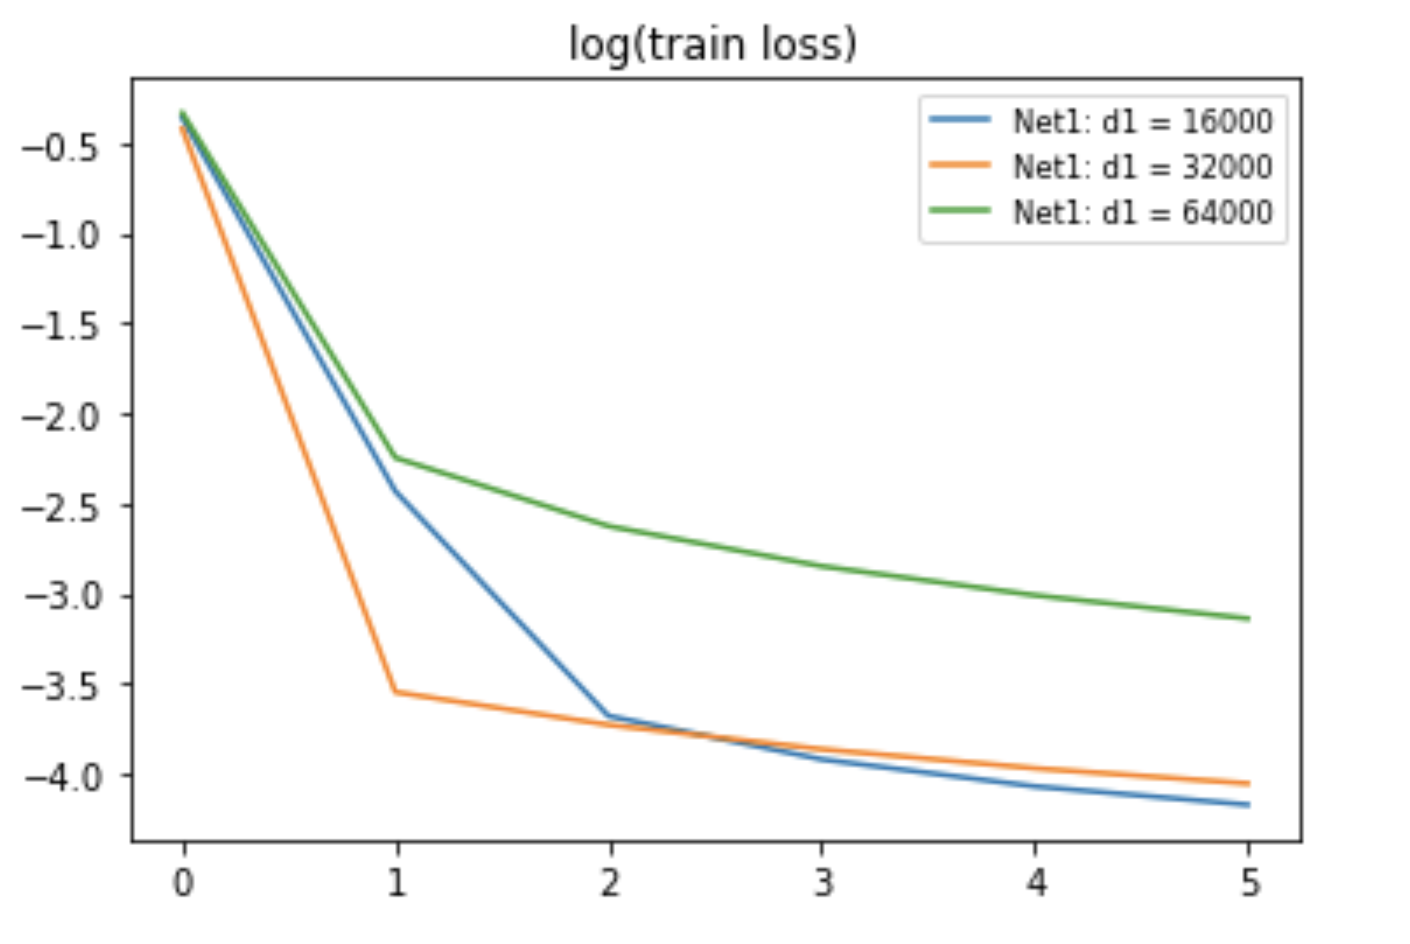
\includegraphics[width=2in]{figure/MNIST_hidden64000_4.png}
	\caption{MNIST: $d_1 = 16000, 32000, 64000$}
\end{figure}

\begin{itemize}
	\item When $d_1 = 1000$, Net1 descend slower than single-layer linear NN from the beginning, but catch up and surpass Net0
	\item When $d_1 > 2000$, Net1 descend faster than Net0 from the beginning. And the speed goes faster as we increase the size of hidden-layer $d_1$.
	\item If we put Net0(Single-layer), NarrowNet1(2-layer with $d_1 = 100$), WideNet1(2-layer with $d_1 = 8000$) together, we can observe that Net0 descend faster at the beginning than NarrowNet1, but NarrowNet1 catches up and surpass Net0 soon. WideNet1 is much more faster than the other two at the beginning and remain the fastest all the time.
\end{itemize}